\section{Neural Style Transfer}

The technique of using neural networks for style transfer is generally referred to as neural style transfer. It is widely acknowledged that the concept of neural style transfer began to gain traction after Gatys et al.\citep{02gatys2016image} utilized convolutional neural networks (CNNs) for style transfer. This paper draws on some of the classification perspectives of neural style transfer discussed in \citep{01jing2019neural}, and based on the current developments in the field and personal understanding, modifies and adds to these perspectives to form a new classification standard for neural style transfer. The new classification standard is primarily based on three criteria: the developmental stages of neural style transfer, the main issues explored at different stages, and the different approaches to solving these issues.

Under this standard, this paper divides neural style transfer into three developmental stages:
\begin{enumerate}
    \item Early Stage: Online style transfer based on pixel iteration, led by Gatys et al. \citep{02gatys2016image}.
    \item Developing Stage: Offline style transfer based on model iteration, led by Johnson et al.\citep{22johnson2016perceptual} and Ulyanov et al.\citep{23ulyanov2016texture}.
    \item Current Stage: Arbitrary and efficient style transfer.
\end{enumerate}

Dividing neural style transfer into these three stages reflects more effectively the developmental trajectory of the field of neural style transfer, allowing researchers to clearly understand the reasons for the emergence of each stage, the main issues being explored, and the solutions proposed. It is important to note that the chronological classification used in this paper may not always accurately place certain works within a specific stage, as some contributions lie at the intersection of two stages and exhibit characteristics of both. In such cases, this paper classifies them into the earlier stage to highlight their connection to preceding work.

Each of the three stages mentioned above has corresponding subcategories. For online style transfer based on pixel iteration, it can be further categorized into two types based on the type of loss function used: style transfer based on parametric models and style transfer based on non-parametric models. For offline style transfer based on model iteration, it can be classified according to the network and the number of styles that can be transferred by the network, resulting in two subclasses: single-network model generating single style, and single-network model generating multiple styles. For arbitrary and efficient style transfer, based on the different technologies used to achieve style transfer, it can be divided into two categories: those that build their own network frameworks and those that use other emerging technologies as support.

This paper will introduce the contributions of each stage of neural style transfer according to the above classification standard. For each contribution, the paper will first provide a brief introduction to its underlying concept, followed by an analysis of its advantages and disadvantages, leading into the next contribution. The categories of neural image style transfer is illustrated as Figure \ref{fig1}

\subsection{Pixel-Iterative Online Style Transfer}

Pixel-iterative online style transfer can be traced back to the research of Alexander et al. \citep{24mordvintsev2015inceptionism} on Convolutional Neural Networks (CNNs). Alexander et al. \citep{24mordvintsev2015inceptionism} aimed to investigate why CNNs have the ability to extract image features. To this end, they inverted a CNN and used the inverted CNN to reverse-engineer the feature maps extracted by the original CNN, attempting to reconstruct an image similar to the original one. As described by Alexander et al. in their paper \citep{24mordvintsev2015inceptionism}, they were able to generate images with "certain artistic characteristics" through this method, as illustrated in Figure \ref{fig2}.


\begin{figure}[htbp]%% placement specifier
    %% Use \includegraphics command to insert graphic files. Place graphics files in 
    %% working directory.
    \centering%% For centre alignment of image.
    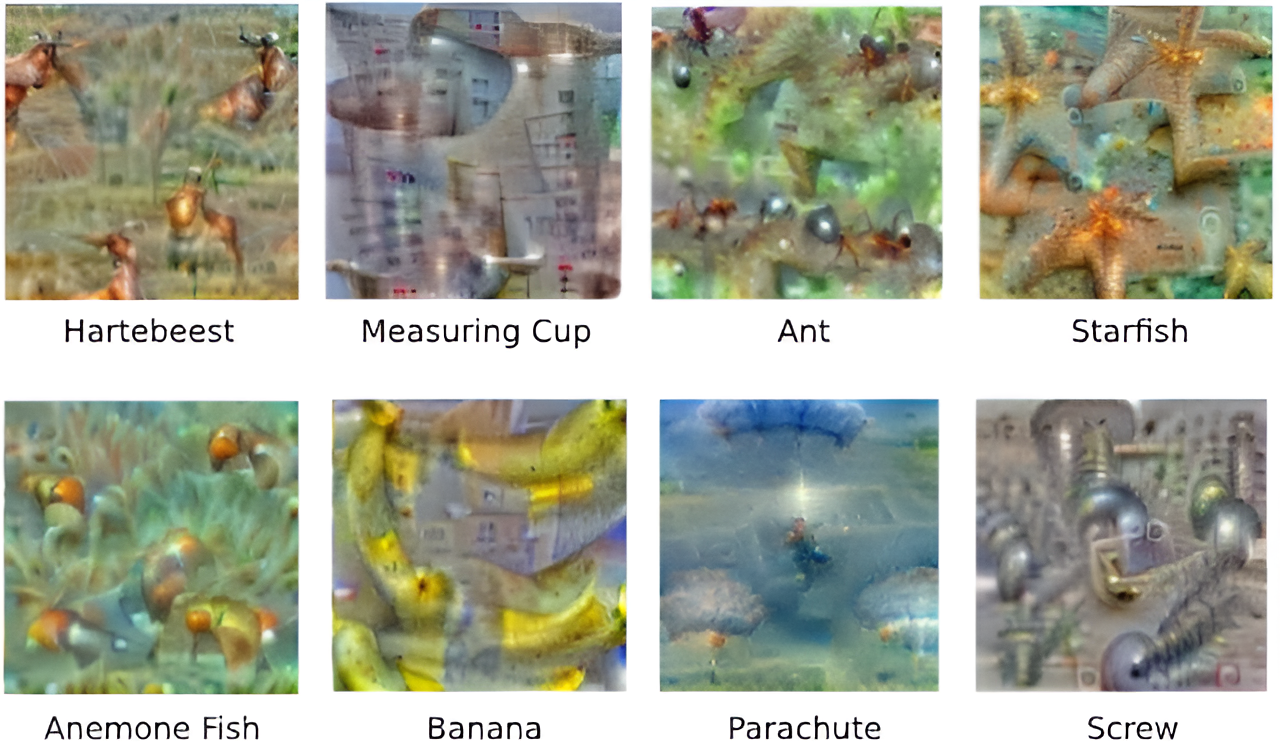
\includegraphics[width=0.95\textwidth]{fig/Alex_classvis.png}
    %% Use \caption command for figure caption and label.
    \caption{The Artistic Images Generated by Alexander et al.\citep{24mordvintsev2015inceptionism}}\label{fig2}
    %% https://en.wikibooks.org/wiki/LaTeX/Importing_Graphics#Importing_external_graphics
\end{figure}


Through the aforementioned experiment, DeepDream discovered that CNNs could not only extract image features but also generate images. This concept of "using neural networks for feature extraction followed by other methods for image generation" laid a foundational groundwork for the subsequent use of neural networks in style transfer.

Following DeepDream, Gatys et al. \citep{02gatys2016image} in 2016 combined deep learning with style transfer in a groundbreaking manner, significantly advancing the effectiveness of style transfer and reaching new heights in visual quality.

This paper posits that if a style transfer method uses a content image and a style image as inputs, and iteratively processes a noise image at the pixel level during the generation of a stylized image, resulting in the final output of a stylized image, then this approach can be classified as pixel-iterative style transfer. Furthermore, depending on the implementation method, this category can be further subdivided into parametric model-based style transfer and non-parametric model-based style transfer.

\subsubsection{Parameterized Model-Based Style Transfer}

The work of Gatys et al. \citep{02gatys2016image} can be regarded as the first use of a parametric model for style transfer, and it is also considered the first significant achievement in the entire field of neural style transfer.

In their 2016 paper\citep{02gatys2016image}, Gatys et al. were the first to combine Convolutional Neural Networks (CNNs) with style transfer. The idea behind this achievement originated from the discovery of Gatys et al. during their research on CNNs: a CNN trained with sufficient data can extract features across different datasets\citep{02gatys2016image}. In the realm of style transfer, this capability of CNNs to extract features can be used to capture the content features of a photograph as well as the style features of an artwork. Figure \ref{fig3_VGGs_Ability} illustrates how the VGG16 image classification network, based on CNNs, is capable of extracting both content and style features at different layers of the network.

\begin{figure}[!htbp]%% placement specifier
    %% Use \includegraphics command to insert graphic files. Place graphics files in 
    %% working directory.
    \centering%% For centre alignment of image.
    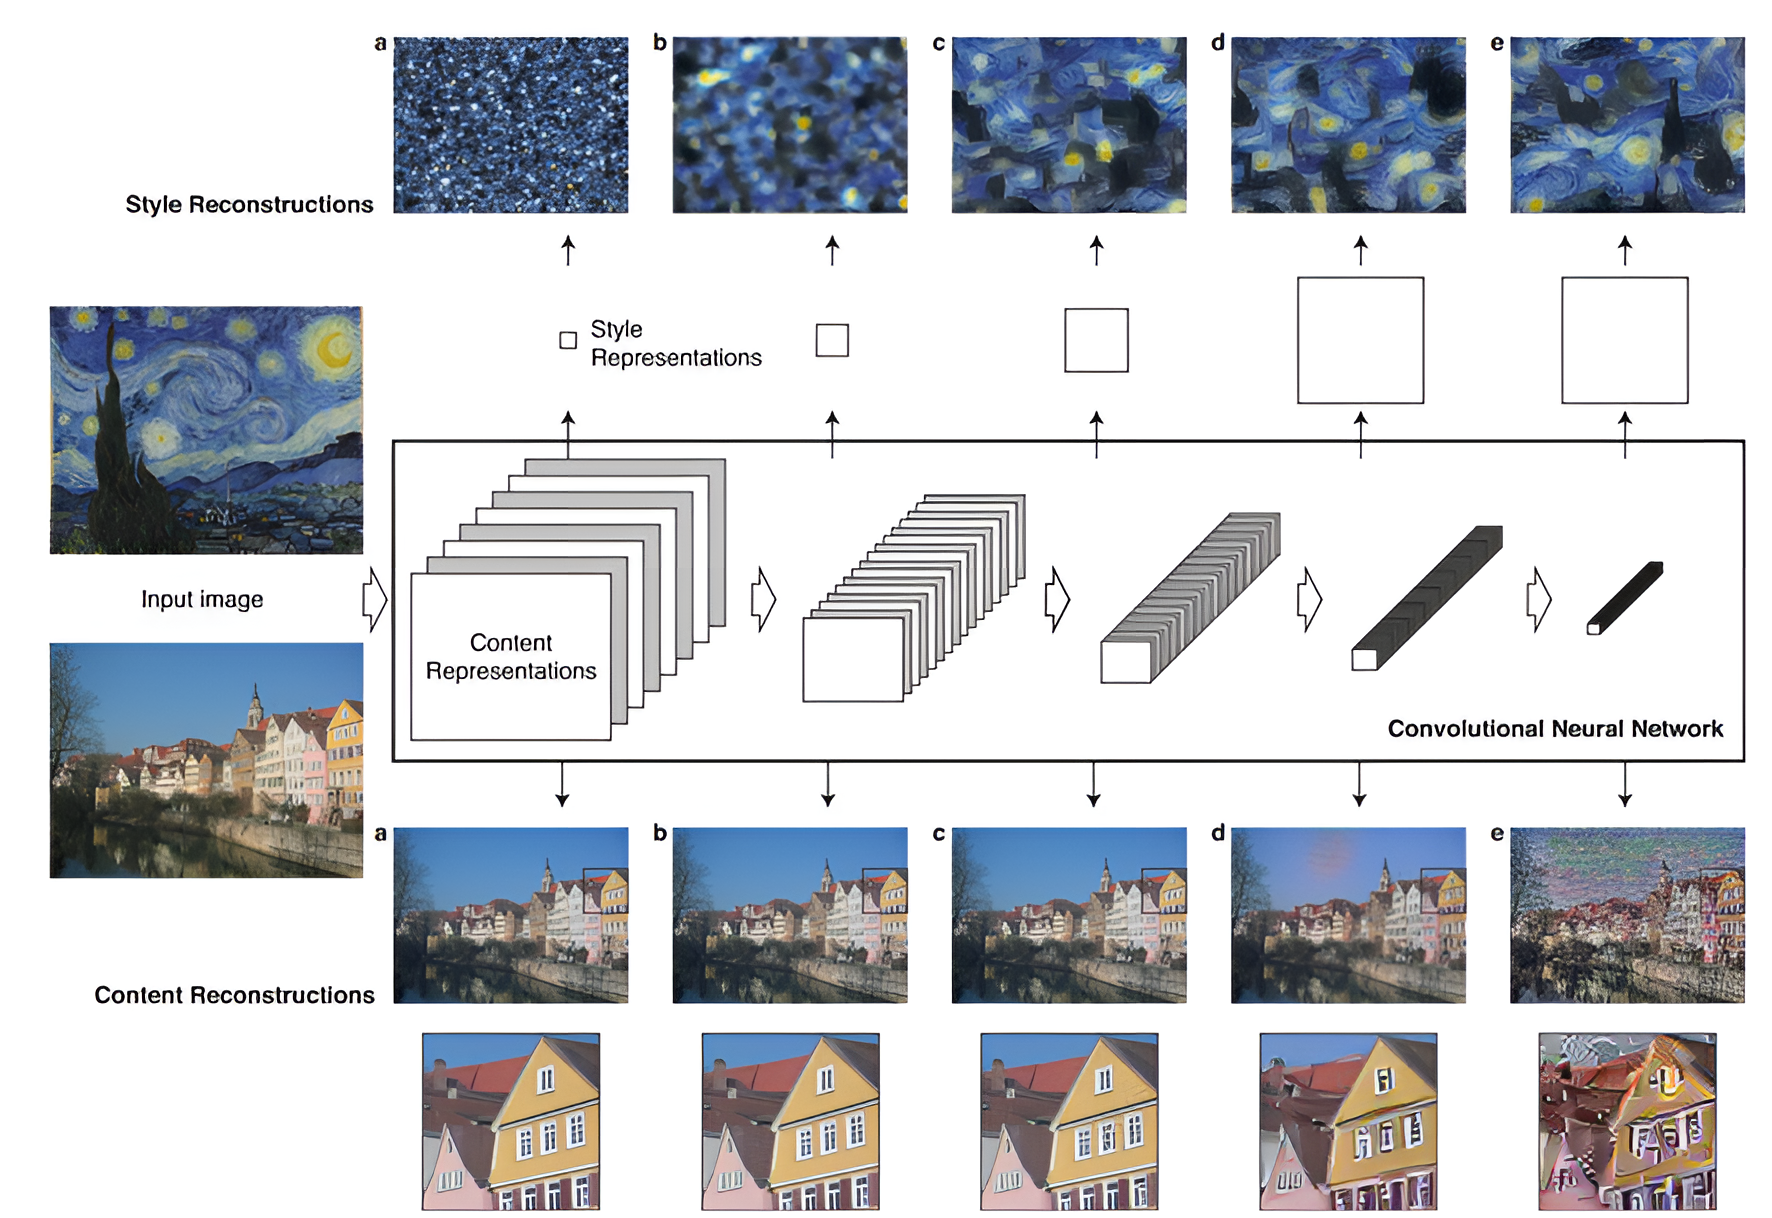
\includegraphics[width=0.95\textwidth]{fig/VGGs_Ability.png}
    %% Use \caption command for figure caption and label.
    \caption{CNN Can Extracting Both Content and Style Features}\label{fig3_VGGs_Ability}
    %% https://en.wikibooks.org/wiki/LaTeX/Importing_Graphics#Importing_external_graphics
\end{figure}

In terms of practical implementation, Gatys et al.\citep{02gatys2016image} achieved style transfer by defining a loss function and using it to optimize a noise image. This loss function is based on the differences between high-level features of the content image and the image being stylized, as well as the differences between high-level features of the style image and the image being stylized. Guided by this loss function, the noise image is iteratively optimized until the loss function reaches its minimum, resulting in the final stylized image. The specific form of the loss function is as follows:

\begin{equation}
    \label{Gatys_total_loss}
    L_{total}=\alpha L_{content}+ \beta L_{style}
\end{equation}

where $L_{total}$  is the overall loss function, $L_{content}$ is the content loss, which measures the degree of content difference between the stylized image and the content image, and $L_{style}$  is the style loss, which measures the degree of style difference between the stylized image and the style image. $\alpha$ and $\beta$ are hyperparameters used to control the similarity between the generated stylized image and the content image and the style image, respectively. Specifically, the content loss function $L_{content}$  is expressed as follows:

\begin{equation}
    \label{gatys_content_l}
    L_{content}\left(\vec{p},\vec{x},l\right)=\frac{1}{2} \sum_{i,j} \left(F_{ij}^l-P_{ij}^l\right)^2
\end{equation}

where $\vec{p}$ is the flattened input of the content image, input into the network in vector form;$\vec{x}$ is the stylized image, which also needs to be flattened for processing. $l$ represents the $l$-th layer in the network.$F^l$ denotes the set of all feature maps generated by the $l$-th layer of the network for the image undergoing style transfer, and $F_{ij}^l$ refers to the value at position $j$ in the flattened vector of the $i$-th feature map in the set $F^l$ generated by the VGG \citep{25simonyan2014very} network at layer $l$. Similarly, $P^l$ denotes the set of all content feature maps generated by the $l$-th layer of the network for the input content image, and $P_{ij}^l$ refers to the value at position $j$ in the flattened vector of the $i$-th content feature map in the set $P^l$. The formula's purpose is to calculate the pixel-wise difference between the feature maps of the stylized image and the corresponding feature maps of the content image, summing these differences. Gradient descent and other optimization methods are used to minimize this value until it stabilizes at a small value.

On the other hand, before providing the specific expression of the style transfer function $L_{style}$ , it is necessary to introduce its core component—the Gram matrix. To extract the style features of the input image, Gatys et al.\citep{02gatys2016image} used a feature space designed to capture texture information, which is built on the output of any convolutional layer in the network. This feature space is constructed from the correlations between feature maps of different convolutional layers, with these correlations represented by the inner product of the $i$-th and $j$-th vectorized feature maps in the $l$-th layer. This inner product is known as the Gram matrix, denoted as $G^i \in R^{N_l\times N_l}$. The formula for the Gram matrix is as follows:
\begin{equation}
    G_{ij}^l=\sum_k F_{ik}^lF_{jk}^L
\end{equation}

Based on the Gram matrix, Gatys et al.\citep{02gatys2016image} processed the noise image using gradient descent and aimed to minimize the mean squared distance between the Gram matrix of the original image and the Gram matrix of the style image. The contribution of the $l$-th layer in the network to the style loss function $L_{style}$  is as follows:
\begin{equation}
    \label{Gatys_style_loss_l}
    E_l = \frac{1}{4N_l^2M_l^2}\sum_{ij}\left(G_{ij}^l-A_{ij}^l\right)^2
\end{equation}
where $N_l$ represents the number of convolutional kernels in a convolutional layer of the network, which is also the number of feature maps that the layer can generate. $M_l$ is the number of pixels contained in each feature map, numerically equal to the product of the height and width of the feature map.$A_{ij}^l$ and $G_{ij}^l$ represent the pixel values at position $j$ in the $i$-th vectorized feature map at layer $l$ of the network. Formula \ref{gatys_style_l} only computes the contribution of a single layer to the style loss $L_{style}$ . The overall style loss $L_{style}$  is obtained by summing the weighted losses from all layers, with the specific formula as follows:

\begin{equation}
    \label{gatys_style_l}
    L_{style}\left(\vec{a},\vec{x}\right)=\sum_{l=0}^L \omega_l E_l
\end{equation}
where $w_l$ is the weight representing the impact of each layer on the total style loss function, and $L$ is the number of convolutional layers in the network. By taking the partial derivative of Formula \ref{Gatys_total_loss}, $\frac{\partial L_{total}}{\partial \vec{x}}$ is obtained, which can be used as input for optimization algorithms and guide the iterative processing of the stylized image to achieve style transfer.

The parameterized model style transfer method based on the Gram matrix introduced by Gatys et al. has distinct advantages\citep{02gatys2016image}. Compared to traditional style transfer methods, it overcomes the limitations of rigid and less variable brushstrokes and achieves excellent results. It also addresses the limitation of traditional methods being restricted to specific styles, enabling the transfer of natural and stylized textures\citep{01jing2019neural}, thus achieving good transfer results. However, this method has some notable drawbacks. Since style transfer starts from a noise image each time, it requires a significant amount of time for batch processing and performs poorly in real-time style transfer. Additionally, the Gram matrix is more adept at capturing global information of feature maps, leading to unsatisfactory results in extracting regular textures with long-range symmetrical structures\citep{01jing2019neural}. Moreover, unlike traditional methods that ignore high-level semantic information, Gatys et al.\citep{02gatys2016image} considered only high-level semantic information and neglected low-level semantic information, resulting in deficiencies in the fine structure and detail coherence of the synthesized stylized images.

To address the shortcomings of fine texture handling in Gatys et al.'s method, Berger et al.\citep{26berger2016incorporating} proposed horizontal and vertical pixel differences, focusing on examining the differences between each pixel and other pixels in its horizontal and vertical directions. In practice, this method calculates the feature relationships between the pixel located at position $(i, j)$ and pixels at positions $(i,j+\delta)$ or $(i+\delta,j)$ in the feature map, incorporating these into the style loss consideration. This approach allowed Berger et al.\citep{26berger2016incorporating} to achieve effective transfer of symmetric long texture patterns, somewhat compensating for Gatys et al.'s limitations in simulating fine structures and regular textures with long-range symmetry. However, since the method still relies on the Gram matrix as the core of style transfer, it retains some of the shortcomings of Gatys et al., such as inadequate texture detail simulation and unstable style transfer quality.

To investigate the reasons behind the style instability in images generated using the Gram matrix, Risser et al.\citep{27risser2017stable} conducted a further in-depth study of Gatys et al.\citep{02gatys2016image}. Risser et al. proposed that the instability in generated image styles is due to feature maps with different means and variances potentially having the same Gram matrix. Based on this finding, Risser et al. incorporated histograms of feature maps into the style transfer loss function, further optimizing the Gram matrix-based style transfer method. The advantage of this approach is the generation of more stable style images; however, incorporating histograms of feature maps makes the computation more complex, increasing the time required for style transfer and reducing efficiency in batch processing. Moreover, Risser et al. only addressed the stability of generated images, leaving the issue of detailed texture description unresolved.

Li et al.\citep{28li2017demystifying} attempted to explain the principles of neural style transfer using more mature domain knowledge, considering neural style transfer as a special variant of domain adaptation tasks. From this perspective, Li et al. provided a different viewpoint. Domain adaptation tasks are based on the fact that the distributions of source and target data are different, with the goal of training a model on a labeled source domain dataset to predict the target domain data distribution. One method of domain adaptation is to minimize the distribution difference between source and target domain samples, where Maximum Mean Discrepancy (MMD) is a commonly used measure. Analogously, in style transfer tasks, the content image can be considered as the source domain, and the stylize image as the target domain. Li et al. explored the mathematical role of the Gram matrix in style transfer and proved that the process of matching Gram matrices of style images and stylized images (i.e., Formula \ref{Gatys_style_loss_l}) is essentially equivalent to minimizing an MMD with a quadratic polynomial kernel. Therefore, Li et al. proposed that minimizing MMD with other kernels (such as linear, polynomial, or Gaussian kernels) might be useful in style transfer. The main contribution of Li et al. is that they provided a theoretical exploration and clarification of the principles of Gatys et al.\citep{02gatys2016image}.

The aforementioned parameterized model-based neural style transfer methods have some common defects. Due to the loss of low-level information in convolutional neural networks, the transfer results for objects with regular shapes (e.g., man-made objects) often exhibit noticeable distortions. Although Berger et al.\citep{26berger2016incorporating} made contributions in this area, there is still significant room for improvement. Additionally, the style transfer process is time-consuming, requiring substantial time for batch processing of many images, and thus is less efficient in tasks with large numbers of images, such as video style transfer. The generated style is also unstable and lacks temporal consistency.

\subsubsection{Non-Parametric Model-Based Style Transfer}

Markov Random Fields (MRFs) are a primary method used in non-parametric model-based neural style transfer. The use of MRFs for texture synthesis is also a common technique in traditional style transfer methods [29–32]. Li and Wand [33] chose to integrate the traditional MRF-based method into neural style transfer. In their work [33], they combined MRFs with deep convolutional neural networks (dCNNs) and proposed a non-parametric neural style transfer method. They argued that the parameterized style transfer method using Gram matrices only considers differences between pixels and lacks spatial-level constraints on the stylized image, leading to insufficient realism in the generated images. Therefore, Li and Wand replaced the Gram matrix with an MRF regularizer and introduced a new loss function:

\begin{equation}
    L_s=\sum_{l\in {l_s}}\sum_{i=1}^m \mid\mid\Psi_i(F^l(I))-\Psi_{NN(i)}(F^l(I_s))\mid\mid^2
\end{equation}

where $\Psi(F^l(I))$ represents the set of all local patches in the feature map$F^(I)$; $\Psi_i(F^l(I))$ refers to the $i$-th local patch within this set; $\Psi_{NN(i)}$ is the style patch in the stylized image $I$ that most closely matches the $i$-th local patch in terms of style similarity. This best-matching stylized patch $\Psi_{NN(i)}$ can be found by calculating the normalized correlation between all style patches in the style image. Here, $m$ denotes the total number of local patches. The method proposed by Li and Wand improved upon the style transfer results achieved by Gatys et al.[2], making the structures in the stylized images more coherent and better preserving the fine details of the original image, leading to significant progress in synthesizing realistic photos. However, this method lacks attention to the semantic content of the images. If there is a substantial structural difference between the content and style images, the matching between local patches and style patches might not be accurate, resulting in poor quality of the generated stylized images.

\textbf{Summary}\quad The pixel-iteration-based style transfer methods can be considered as early explorations in the field of neural style transfer, holding a pioneering position.
Neural style transfer technology overcomes the limitation of traditional style transfer techniques, which only transfers a single style. It has better generalization ability, achieving a "once-for-all" approach to some extent, meaning that once a network structure is built, it can transfer any style and handle images of any resolution. Additionally, thanks to the CNN's feature extraction capabilities, neural style transfer can capture advanced artistic styles and textures, exhibiting flexible and diverse texture features within the same stylized image.
However, despite the groundbreaking achievements of pixel-iteration-based style transfer, some common issues cannot be ignored, with the most critical being resource consumption and time expenditure. Pixel-iteration-based style transfer requires multiple iterations of a noise image under the guidance of a loss function, with each iteration involving feature extraction and computation by a CNN. As a result, a significant amount of computational resources and time is consumed during the image generation stage. For instance, when transferring the style of a $512\times 512$ image to generate a similarly sized stylized image, the process can take up to 51.19 seconds\citep{01jing2019neural}. If one attempts to transfer a high-resolution (e.g., 4K) image, the time required becomes even more prohibitive for practical applications.
Moreover, even after investing substantial time and computational resources in style transfer, it is often difficult to consistently achieve results that surpass those of traditional style transfer methods.
These two major drawbacks have hindered the widespread application of neural style transfer technology in real-world scenarios, leading to a stagnation in the research of neural style transfer. 


